\providecommand{\main}{../../..}
\documentclass[\main/dresen_thesis.tex]{subfiles}
\renewcommand{\thisPath}{\main/chapters/largeScaleInstruments/laboratoryInstruments}
\begin{document}

\section{Laboratory Instruments}
  \subsection{PPMS Evercool II - VSM}
    \label{ch:instruments:laboratoryInstruments:vsm}
    \begin{figure}[ht]
      \centering
      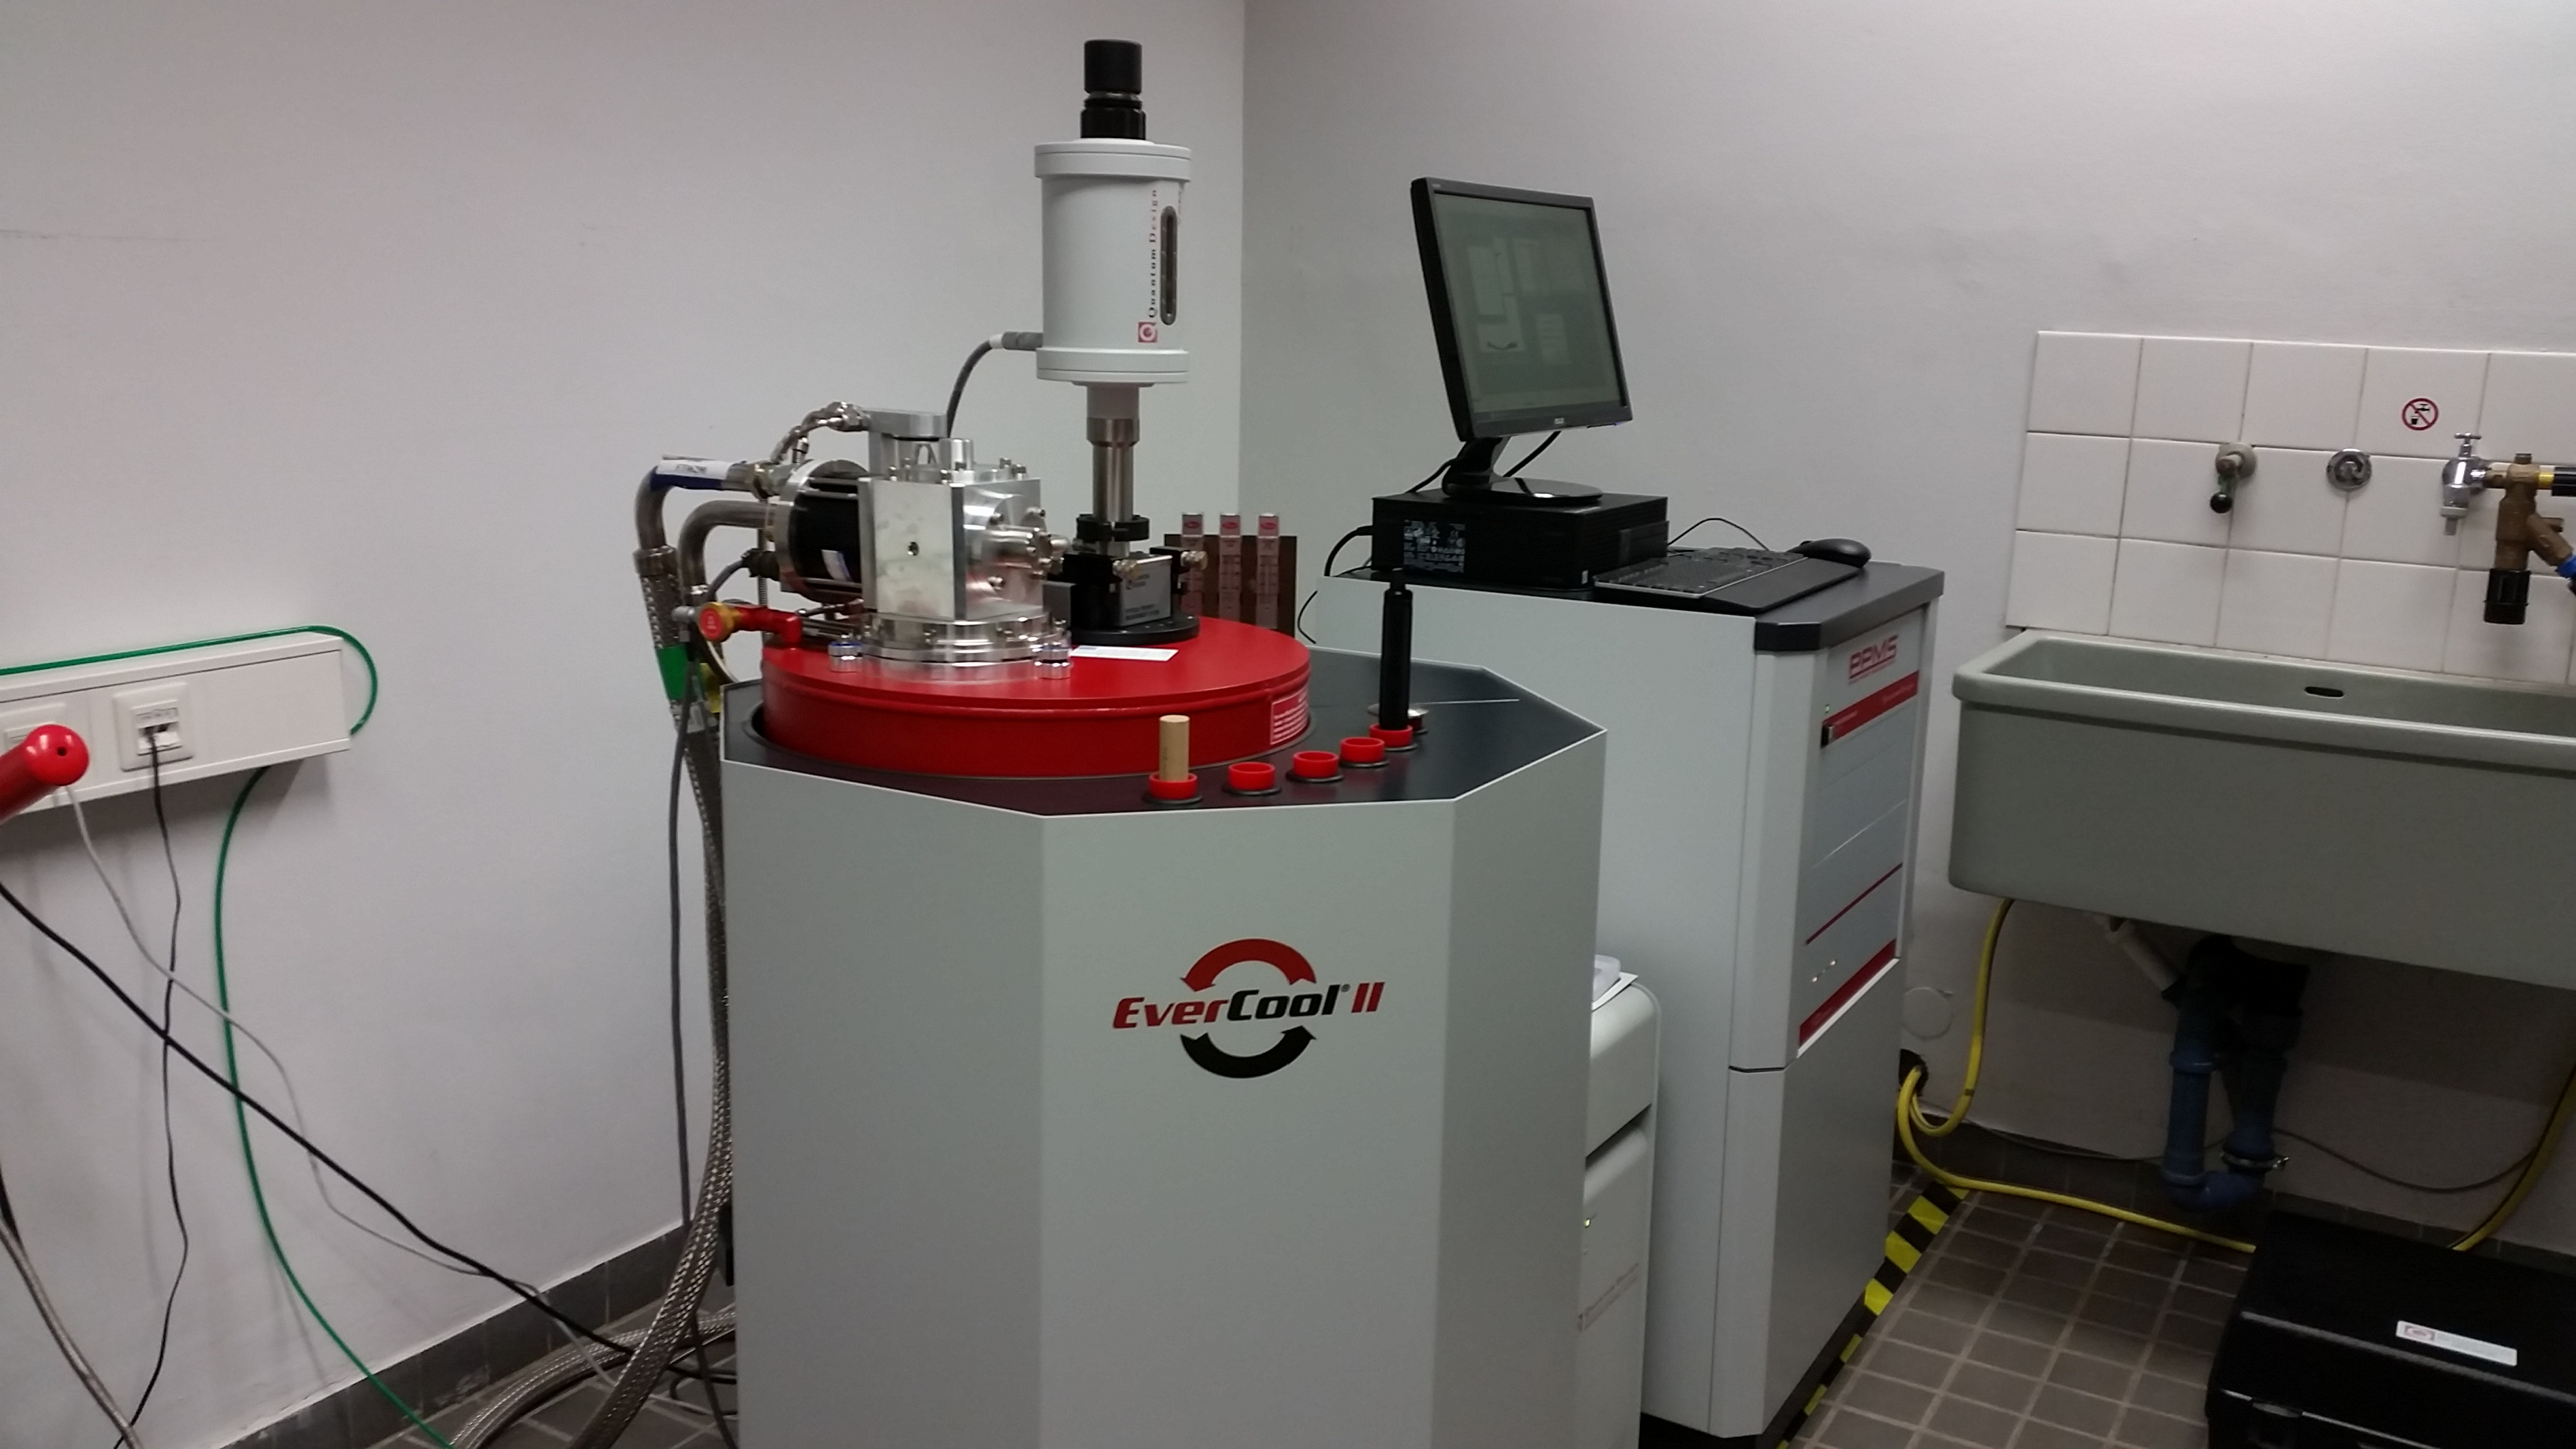
\includegraphics[width=0.7\textwidth]{instruments_ppms}
      \caption{\label{fig:appendix:instruments:ppms}The physical property measurement system (PPMS) Evercool II, which is used to measure the macroscopic magnetization properties by vibrating sample magnetometry.}
    \end{figure}
    During the course of this thesis a PPMS Evercool II from the company LOT Quantum Design was set up in the working group.
    The preparation of the laboratory for the instrument and support of the installation was performed in parallel to this thesis.

    The installed Evercool II has the option to choose between VSM (\refch{ch:methods:vsm}) and AC-Susceptometry, where the latter was not utilized in the scope of this thesis.
    An external field of up to $\pm 9 \unit{T}$ can be applied to magnetize samples, which are up to $5 \unit{mm}$ in diameter.
    Additionally the temperature can be freely varied in a temperature range of $2 \ldots 400 \unit{K}$.
    The instrument control is performed using the MultiVu software of LOT QuantumDesign.

    The Evercool II has a closed helium cycle.
    Meaning that only Helium lost during sample change or due to over-pressure from fast temperature/field changes needs to be refilled.
    To cool the Helium compressor of the helium cycle, a water-cooling solution has been installed.

    For a measurement on the Evercool II, samples on a substrate are fixed on Quartz holders provided by QuantumDesign (QD-P125B) by using a low temperature varnish by GE (GE 7031).
    Liquid samples on the other hand are sealed vacuum-tight in custom-built glass vials of the company Hilgenberg, which can be fixed in a colorless drinking straw for insertion into the PPMS.
    The sealing of the glass vial is done by first freezing the liquid on a thermoelectric cooler, then putting the vial on underpressure by using a suction pump and finally by using a hydrogen burner to melt a stricture and rotating it simultaneously, which causes the glass to collapse inward and seal the vial tight.
    The magnetization of the samples is then measured at a pressure of $25 - 33 \unit{mBar}$, while sweeping either the magnetic field between $\pm 9 \unit{T}$ or the temperature from $10 - 350 \unit{K}$.
    The VSM option has a noise level in the order of $0.3 \ldots 4 \unit{\musf emu}$, depending on the temperature and external field.


  \subsection{D8 Advanced - XRR}
    \label{ch:instruments:laboratoryInstruments:xrr}
    \begin{figure}[ht]
      \centering
      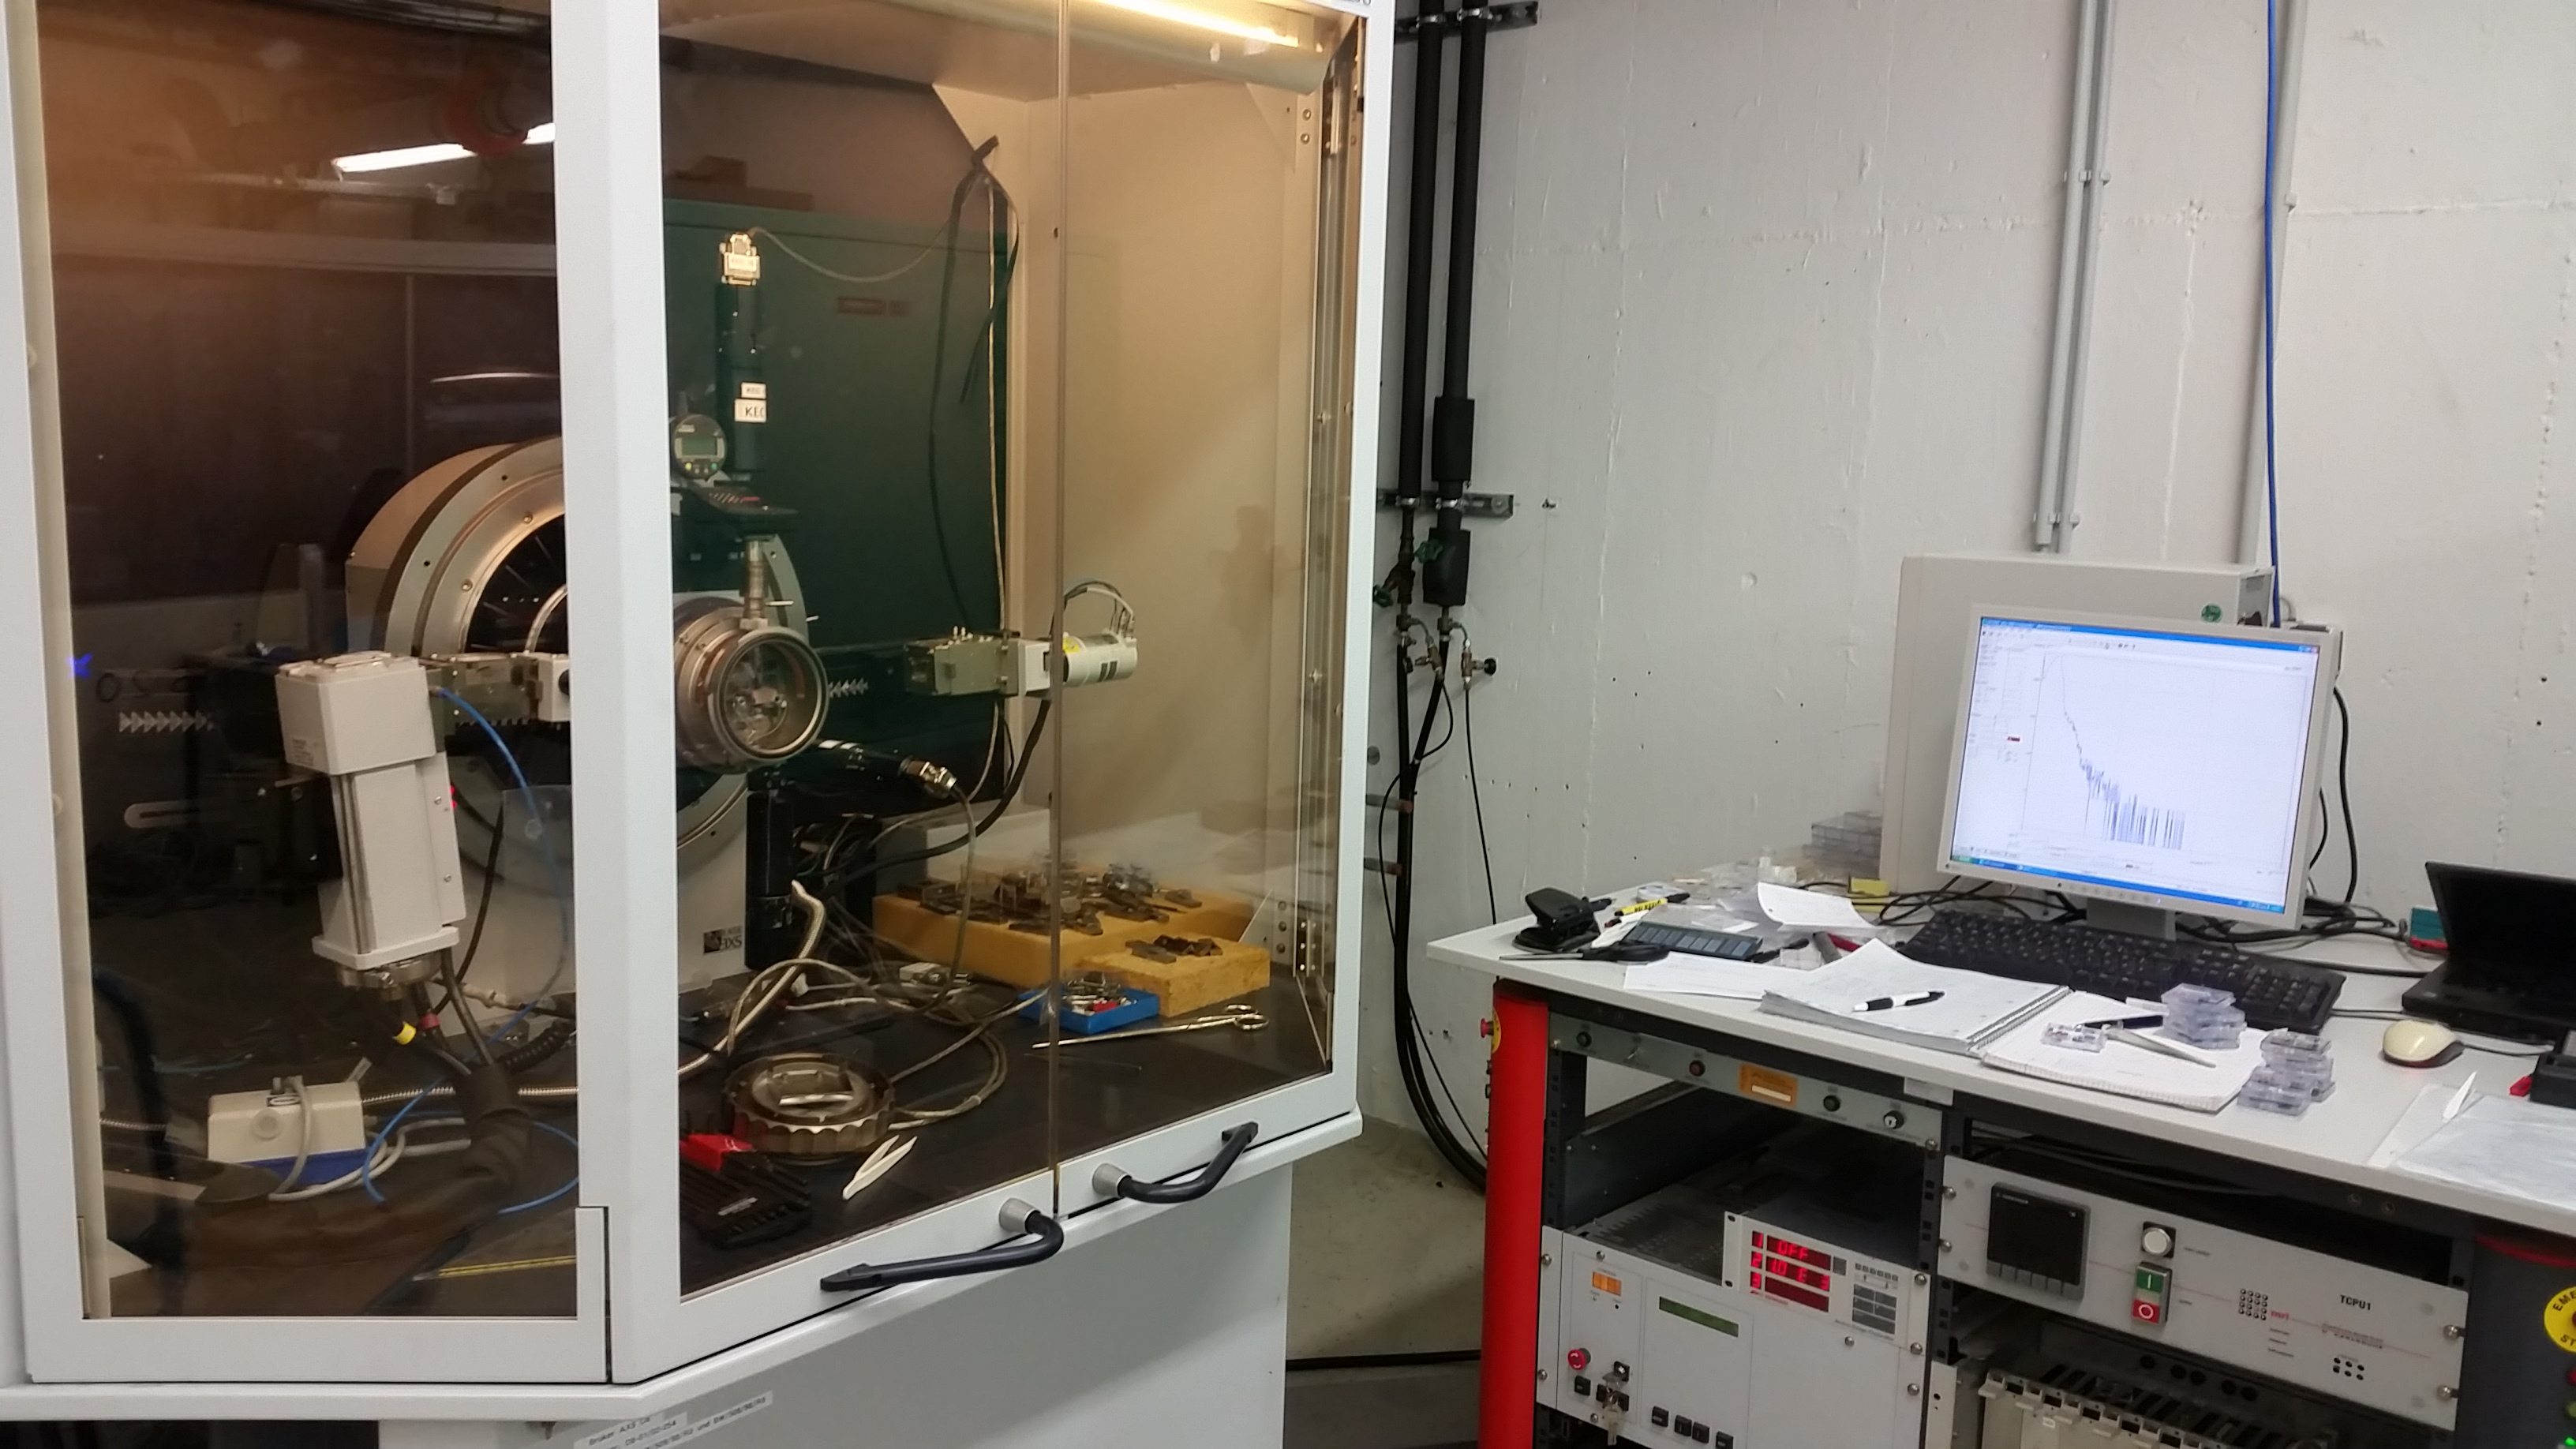
\includegraphics[width=0.7\textwidth]{instruments_brukerD8}
      \caption{\label{fig:appendix:instruments:brukerD8}Bruker D8 instrument, which can be used for X-ray reflectometry and X-ray diffraction.}
    \end{figure}
    To perform XRR experiments, described in \refch{ch:methods:xrr}, a D8 Advanced instrument from the company Bruker was used at the \textsc{Forschungszentrum J\"ulich}.
    The D8 operates with a Cu-K$\alpha$ source ($\lambda \eq 1.54 \unit{\angstrom}$) and has two G\"obel mirrors installed to direct the beam in front and after the sample.
    The source and the detector are both installed at a fixed distance of approximately $30 \unit{cm}$ from the sample position in a Bragg-Brentano geometry, where the sample is fixed while source and detector are both moved.
    At the source and detector, slits of $0.2 \unit{mm}$ width are installed.
    Additionally, absorber materials can be placed in the beam path electronically, in case the photon count on the detector is larger than the electronics can handle, \eg when the transmission of the direct beam is measured.

    \begin{figure}[ht]
      \centering
      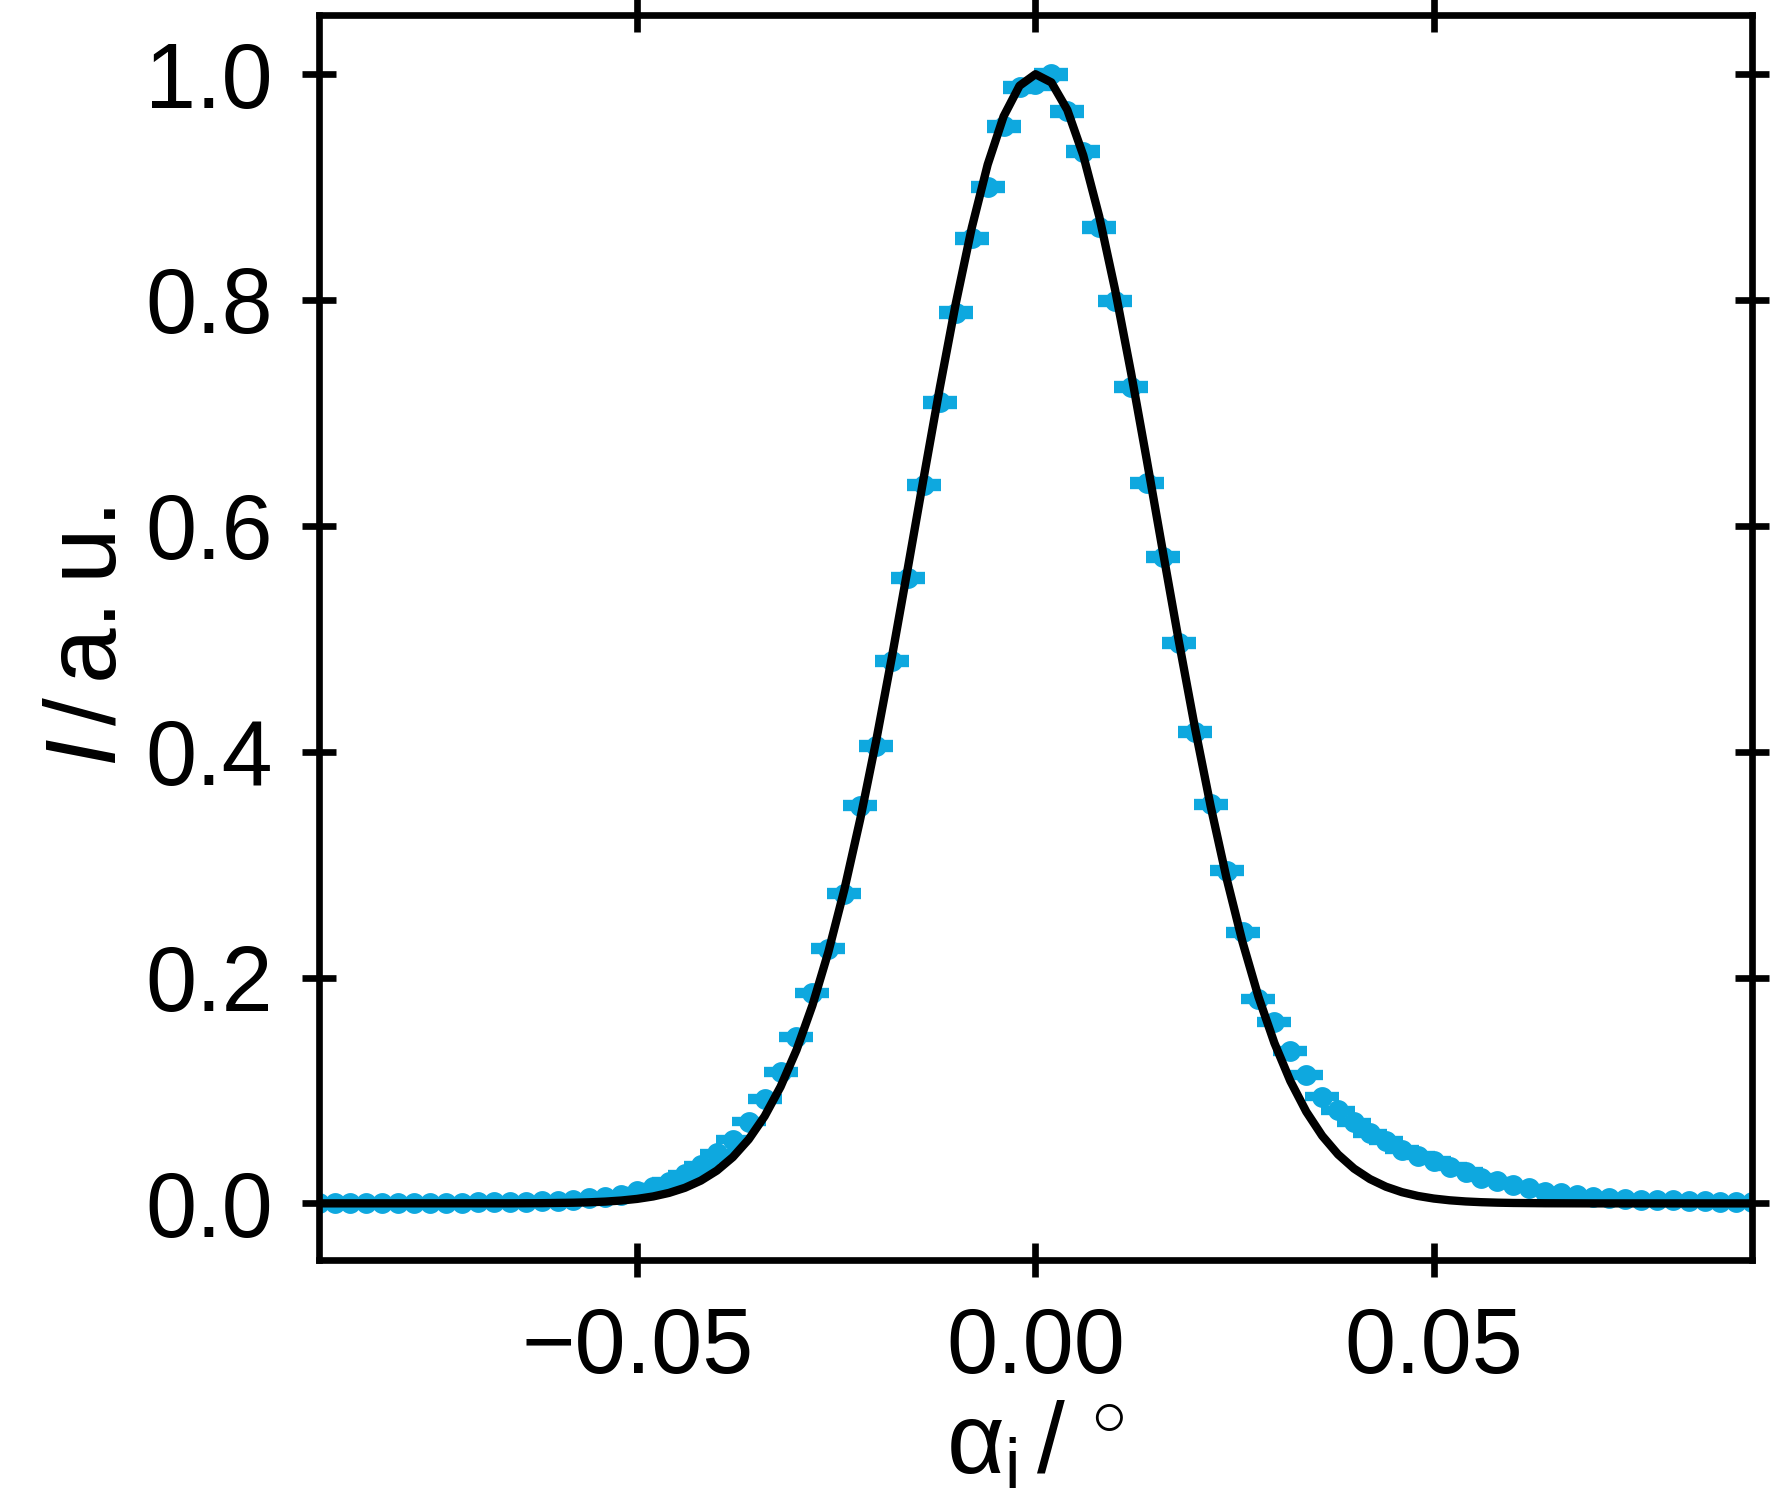
\includegraphics{appendix_instruments_brukerD8DirectBeam}
      \caption{\label{fig:appendix:instruments:brukerD8DirectBeam}Direct beam scan of the D8 instrument at a beam slit size of $0.2 \unit{mm}$, modeled by a Gaussian function to estimate the divergence.}
    \end{figure}

    By scanning the direct beam of the instrument, when no sample is placed in the beam path, the angular divergence is estimated as shown in \reffig{fig:appendix:instruments:brukerD8DirectBeam}.
    The best fit with a Gaussian function results in a divergence of $\Delta \alpha_i \eq 0.01510(4) ^\circ \eq 2.635(7) \cdot 10^{-4}$, which corresponds for the distance of $30 \unit{cm}$ to a width of $0.15 \unit{mm}$, which is in the order of magnitude of the slit size.


  \subsection{X'Pert PRO - XRD}
    \label{ch:instruments:laboratoryInstruments:xrd}
    XRD measurements (\refch{ch:methods:xrd}) were performed by a collaboration with the group of Daniel Nižňanský from the Department of Inorganic Chemistry at the Charles University in Prague.
    An X'Pert PRO instrument from the company PANalytical was used for this purpose and the data was acquired using a Cu K$\alpha$ source ($\lambda \eq 1.54 \unit{\angstrom}$) and a PIXcel detector.
    The instrument has a Bragg-Brentano geometry analogue to the D8 Advanced instrument, which was used for XRR.

    For the measurement, a concentrated dispersion of the nanoparticle of interest is dried on a glass substrate and the measured scattering angle range is in all cases set to $2 \theta \eq 5 \ldots 80^\circ$, which corresponds to a $q$-range of $1 \ldots 5 \unit{\angstrom^{-1}}$.


  \subsection{Neon Zeiss 40 - SEM}
    \label{ch:instruments:laboratoryInstruments:sem}
    \begin{figure}[ht]
      \centering
      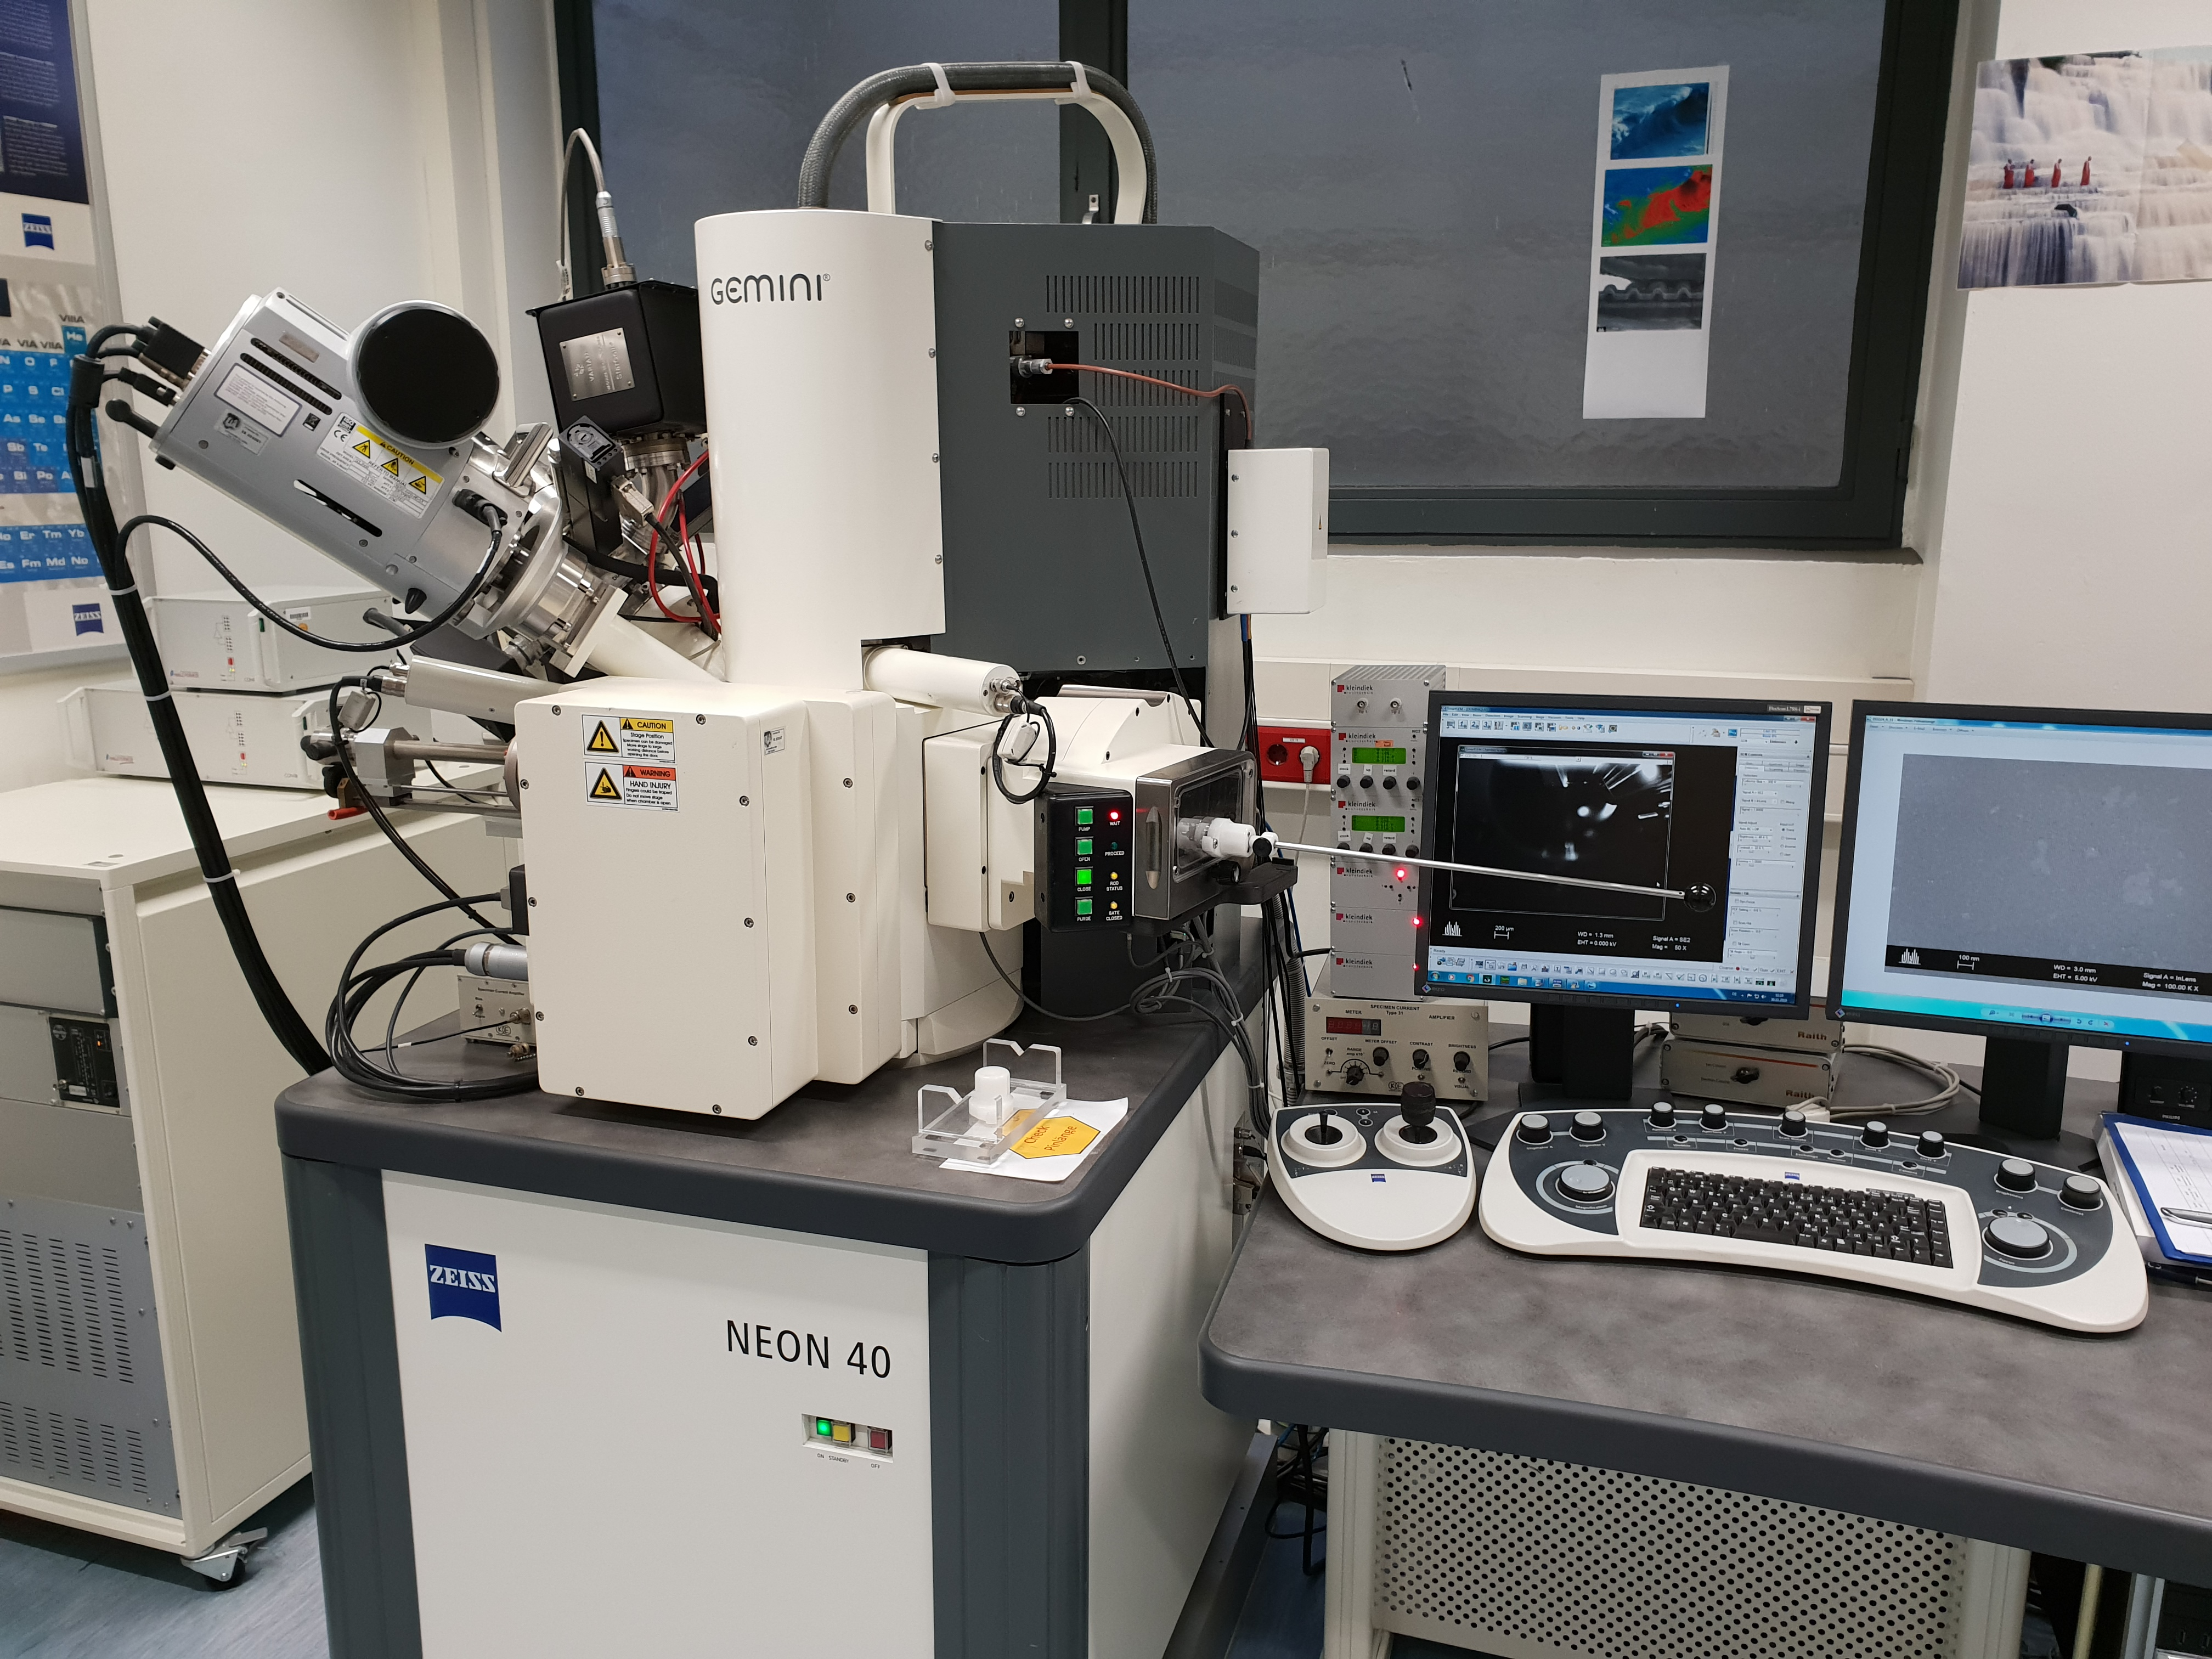
\includegraphics[width=0.7\textwidth]{instruments_laboratoryInstruments_sem}
      \caption{\label{fig:appendix:instruments:sem}Scanning electron microscope Neon Zeiss 40 used to obtain micrographs of the local nanostructure.}
    \end{figure}
    To obtain micrographs of the nanostructures by scanning electron microscopy, a Neon Zeiss 40 instrument was operated.
    Here, thin nanoparticle layers on silicon substrates are inserted and measured using a primary electron beam at $5 \unit{kV}$ in high-vacuum ($< 10^{-4} \unit{mbar}$).
    In the shown micrographs of this thesis, the intensity of the back-scattered electrons is showed as detected by the InLens detector of the instrument.
    The samples are placed for this purpose at a distance of $3 - 5 \unit{mm}$ to the electron beam exit by controlling the three-dimensional movable sample stage with a joystick.
    Varied positions of the sample are then scanned using the pixel average mode to focus the beam, and the noise reduced micrographs are then finally measured in a slower line average mode for evaluation.
    The micrographs are obtained in the TIF file format, which is loaded for evaluation with the Fiji software \cite{Schindelin_2012_Fijia} or into a Python script using a Java bridge with the Bioformats package \cite{Linkert_2010_Metad}.

  \subsection{Zeiss LEO 902 - TEM}
    \label{ch:instruments:laboratoryInstruments:tem}
    Transmission electron microscopy experiments were carried out on a Zeiss Leo 902 microscope operating at $120 \unit{kV}$ with a \ch{LaB6} cathode in bright field mode to obtain high-magnification micrographs of individual nanoparticles.
    The diluted nanoparticle dispersion of interest is deposited on a copper grid, which is then inserted into the TEM.
    Finally, multiple positions of the grid are measured at varied magnifications to obtain micrographs in the TIF file format, which are evaluated with the same software as the SEM micrographs in \refsec{ch:instruments:laboratoryInstruments:sem}.
\end{document}
